\setAuthor{Valter Kiisk}
\setRound{piirkonnavoor}
\setYear{2009}
\setNumber{G 4}
\setDifficulty{2}
\setTopic{Elektriahelad}

\prob{Elektriküünlad}
Jõulukaunistuse valmistamiseks otsis Juku välja 10
taskulambipirni (nimipinge \SI{3}V, võimsus \SI{0.6}W) ja alaldi klemmipingega \SI{5}V.
Seejärel koostas ta skeemi, mis on kujutatud joonisel.\\
\osa Kui suur peab olema
takisti $R$ takistus, et pinge lampidel ei ületaks nimipinget?\\
\osa Skeemi sisselülitamisel avastas Juku, et lambid põlevad oodatust tuhmimalt. Selgus, et alaldi
klemmipinge oli koormusega langenud \SI{4}V-ni ning pinge lampidel \SI{2,3}V-ni. Kui suur
tuleks valida takisti $R$ väärtus, et lambid põleksid normaalse heledusega?

\begin{center}
	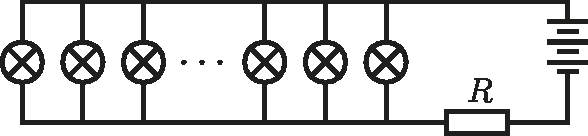
\includegraphics[width=0.8\linewidth]{2009-v2g-04-yl}
\end{center}

\hint
\osa Takisti peab tagama selle, et lampide pinge ei ületaks nominaalpinget ükskõik missuguse lambi sisetakistuse väärtuse korral\\
\osa Lampide oodatavast tuhmimalt põlemine on põhjustatud alaldi sisetakistusest.

\solu
\osa Lambi nimivool on $\SI{0,6}W/\SI{3}V=\SI{0,2}A$. 10
lampi tarbivad voolu $10\times \SI{0,2}A=\SI{2}A$. Pingelang takistil on $\SI{5}V-\SI{3}V=\SI{2}V$. Järelikult vajalik takistus on $\SI{2}V/\SI{2}A=\SI{1}{\ohm}$.

\osa \SI{1}{\ohm}-st takistit kasutades oli voolutugevus ahelas $(\SI{4}V-\SI{2,3}{V})/\SI{1}{\ohm}=\SI{1,7}A$. Sellise koormuse tulemusel langes pinge vooluallika
klemmidel \SI{1}V võrra, seega alaldi sisetakistus on $\SI{1}V/\SI{1,7}A=\SI{0,59}{\ohm}$. Järelikult takisti $R$ takistuse sobilik väärtus oleks
$\SI{1}{\ohm}-\SI{0,59}{\ohm}=\SI{0,41}{\ohm}$.
\probend